\documentclass[12pt,a4paper,titlepage,ngerman,pdftex]{report}
\usepackage[utf8]{inputenc}
\usepackage[german]{babel}
\usepackage[T1]{fontenc}
\usepackage{amsmath}
\usepackage{amsfonts}
\usepackage{amssymb}
\usepackage{graphicx}
\usepackage{acronym}
\usepackage{setspace}
\usepackage{geometry}
\usepackage{caption}
\usepackage{subcaption}
\usepackage{hyperref}
\usepackage{listings}
\usepackage{textcomp}
\geometry{a4paper, top=25mm, left=25mm, right=25mm, bottom=25mm,
    headsep=10mm, footskip=12mm}
\usepackage{xcolor}

\definecolor{mygreen}{rgb}{0,0.6,0}
\definecolor{mygray}{rgb}{0.5,0.5,0.5}
\definecolor{mymauve}{rgb}{0.58,0,0.82}
\definecolor{backcolour}{rgb}{0.827, 0.827, 0.827}
\definecolor{dkblue}{rgb}{0,0,.6}
\definecolor{dkyellow}{cmyk}{0,0,.8,.3}

\lstset{
    language        = php,
    basicstyle      = \small\ttfamily,
    keywordstyle    = \color{dkblue},
    stringstyle     = \color{red},
    identifierstyle = \color{mygreen},
    commentstyle    = \color{gray},
    emph            =[1]{php},
    emphstyle       =[1]\color{black},
    emph            =[2]{if,and,or,else},
    emphstyle       =[2]\color{dkyellow}}

\lstset{ %
    backgroundcolor=\color{backcolour},   % choose the background color
    basicstyle=\footnotesize,        % size of fonts used for the code
    breaklines=true,                 % automatic line breaking only at whitespace
    captionpos=b,                    % sets the caption-position to bottom
    commentstyle=\color{mygreen},    % comment style
    escapeinside={\%*}{*)},          % if you want to add LaTeX within your code
    keywordstyle=\color{blue},       % keyword style
    stringstyle=\color{mymauve},     % string literal stylebreakatwhitespace=false,
    keepspaces=true,
    numbers=left,
    numbersep=5pt,
    showspaces=false,
    showstringspaces=true,
    showtabs=false,
    tabsize=2
}

\begin{document}
%%%%%%%%%%%%%%%%%%%%%%%%%%%%%%%%%%%%%%%%%%%%%%%
%%%%%%%%%%%%%%%%%    TITLE    %%%%%%%%%%%%%%%%%
%%%%%%%%%%%%%%%%%%%%%%%%%%%%%%%%%%%%%%%%%%%%%%%
    \begin{titlepage}
        \centering
        %\includegraphics[width=0.15\textwidth]{pic/picsim_logo_full.png}\par\vspace{1cm}
        {\scshape\LARGE Duale Hochschule Baden-Württemberg \par}
        \vspace{1cm}
        {\scshape\Large Advanced Software Engineering 2 \\--\\ Dokumentation\par}
        \vspace{1.5cm}
        {\huge\bfseries Bierwart\par}
        \vspace{2cm}
        {\Large\itshape Levin Baumann, Marius Holwein\par}
        \vfill
        Dozent\par
        Daniel \textsc{Lindner}

        \vfill

% Bottom of the page
        {\large \today\par}
    \end{titlepage}

%%%%%%%%%%%%%%%%%%%%%%%%%%%%%%%%%%%%%%%%%%%%%%%
%%%%%%%%%%%%%%%%%  LISTINGS  %%%%%%%%%%%%%%%%%
%%%%%%%%%%%%%%%%%%%%%%%%%%%%%%%%%%%%%%%%%%%%%%%
    \pagenumbering{Roman}
    \tableofcontents
    \listoffigures
    \lstlistoflistings

%%%%%%%%%%%%%%%%%%%%%%%%%%%%%%%%%%%%%%%%%%%%%%%
%%%%%%%%%%%%%%%%%  Acronym  %%%%%%%%%%%%%%%%%
%%%%%%%%%%%%%%%%%%%%%%%%%%%%%%%%%%%%%%%%%%%%%%%
    \chapter*{Abkürzungsverzeichnis}
    \begin{acronym}[all]
        \acro{dhbw}[DHBW]{Duale Hochschule Baden-Württemberg}
        \acro{rest}[REST]{REstful State Transfer}
        \acro{api}[API]{Application Programming Interface}
    \end{acronym}
    \onehalfspacing

    \chapter{Projektbeschreibung}\label{ch:projektbeschreibung}
    Der Bierwart, im Rahmen dieser Abgabe, ist eine reine \ac{rest}-\ac{api}. Es besteht ein separat ausführbares Frontend unter \url{https://github.com/HerrLevin/Bierwart-frontend}.
    Die \ac{api} ist mit Swagger dokumentiert und befindet sich unter \url{http://localhost:8000/swagger/}\footnote{nur nach erfolgreicher Einrichtung beschrieben in \ref{sec:einrichtung} möglich.}.
    Hier lassen sich mit Betätigung des Buttons \textit{Try it out} einzelne Requests ohne Zusatzprogramme ausführen.


    \section{Einrichtung}\label{sec:einrichtung}

    \begin{enumerate}
        \item \texttt{git clone https://github.com/HerrLevin/Bierwart.git}
        \item \texttt{cd Bierwart}
        \item \texttt{composer install}
        \item sqlite-Datenbank in \texttt{database} namens \texttt{database.sqlite} erstellen und\\ \texttt{default\_migration.sql} ausführen
        \begin{itemize}
            \item alternativ \texttt{database.bak.sqlite} in \texttt{database.sqlite} umbenennen
        \end{itemize}
        \item \texttt{php -S localhost:8000} im Hauptverzeichnis
        \item \url{http://localhost:8000/swagger/} aufrufen
    \end{enumerate}


    \chapter{Entwicklung}\label{ch:entwicklung}
    %Idk, was hier alles rein soll

    Für unsere Clean Architecture haben wir drei Schichten geplant.
    Die innerste Schicht mit dem unvorhersehbaren Namen \verb|Core| ist vergleichbar mit der Schicht 2 (Application Code).
    Sie enthält unsere Use Cases, welche sich hinter den Interfaces einzelner Controller finden.
    Wir sind der Meinung eine Getränkeabrechnung wird die von uns implementierten Use Cases immer benötigen und eine Änderung an diesen ist höchst unwahrscheinlich.
    Die Controller dienen hierbei der Übersichtlichkeit.
    Die nächste Schicht sind unsere \verb|Adapter|.
    Sie ist vergleichbar mit der in der Vorlesung beschriebenen Schicht 1 (Adapter).
    Sie enthält die implementierenden Klassen der \verb|Core| Schicht, einen Validator für json Arrays, ein Query Builder Interface für eine Datenbank und die Klasse \verb|DB|, in welcher der Datenbankconnector instanziiert wird.
    Zudem die \verb|Helpers| Klasse für unsere Testingumgebung und das dumpen sowie ein HTTP Router und die Klassen für Request und Response.
    Bei Technologieänderungen lassen sich diese hier durchführen ohne alles wegwerfen zu müssen.
    In dieser Schicht entkoppeln wir unseren Core von der nächsten Schicht, den \verb|Plugins|.
    Unsere Schnittstelle nach außen ist eine REST API.
    Auf diese weise können wir in Zukunft immer den neusten Scheiß als UI nutzen.
    In der äußersten Schicht findet sich die Anbindung an unsere SqLite Datenbank, denn die Welt der Datenbanken ist teilweise sehr rau und wechselhaft.

    \section{Refactoring}\label{sec:refactoring}

    \subsection{Router}\label{subsec:router}
    Der Router des Projektes funktioniert nach einem "First Pattern Matching"-Prinzip.
    Um dies in der Routenkonfiguration leicht umzusetzen, beendet sich die Ausführung des Prozesses, sobald eine Route gefunden und die entsprechende Methode darin ausgeführt wurde.
    Dies geschah anfangs über ein \verb|exit(0);|, was leider untestbar ist.
    Der hier entsprechende Codesmell sind \href{https://refactoring.guru/refactoring/technical-debt}{technische Schulden}, da dieses Codefragment zunächst nur als ungetestetes MVP diente und die Folgen der \glqq Untestbarkeit\grqq{} zunächst nicht bewusst waren.
    Um dieses Problem zu umgehen, ersetzten wir zunächst diese Zeile durch das Werfen einer eigenen Exception: \verb|throw new TaskFailedSuccessfullyException();|\footnote{\url{https://github.com/HerrLevin/Bierwart/commit/b56b8ea86c12fe04e9f5ead235ca783f14aa1910}}

    Diese konnten wir sowohl in unseren Tests abfangen, als auch in unserer \verb|index.php|:

    \begin{lstlisting}[language=php,label={lst:lstlisting},caption={Ursprüngliche Implementation der Router-Exception}]
$request = $_SERVER['REQUEST_URI'];
$router = new Router($request);
try {
    $router->get('/', Bierwart::class, 'getHelloWorld');
    $router->get('/generateReport', ReportsController::class, 'generateReport');

    Router::abort();
} catch (TaskFailedSuccessfullyException) {
//This place is a message... and part of a system of messages... pay attention to it!
//Sending this message was important to us. We considered ourselves to be a powerful culture.
//This place is not a place of honor... no highly esteemed deed is commemorated here... nothing valued is here.
//What is here was dangerous and repulsive to us. This message is a warning about danger.
//The danger is in a particular location... it increases towards a center... the center of danger is here... of a particular size and shape, and below us.
//The danger is still present, in your time, as it was in ours.
//The danger is to the body, and it can kill.
//The form of the danger is an emanation of energy.
//The danger is unleashed only if you substantially disturb this place physically. This place is best shunned and left uninhabited.
}
    \end{lstlisting}
\noindent
    Im weiteren Verlauf, wurde die statische Methode \verb|Helpers::dd();| eingeführt.
    Diese steht für \textit{Dump \& Die} -- sie gibt, sofern mitgegeben, einen Dump einer Variable aus und beendet den aktuellen Prozess.
    Dies hat den Vorteil zur Folge, dass der Aufruf der statischen Methode in Tests mockbar ist.

    Dummerweise hat somit die \verb|TaskFailedSuccessfullyException| dieselbe funktionalität wie \verb|dd()|.
    Der hierfür entsprechende Codesmell ist die \href{https://pragmaticways.com/31-code-smells-you-must-know/#6_Oddball_Solution}{Oddball Solution}.
    Deshalb haben wir die ungewöhnlichere und technisch teurere Funktionalität der Exception ausgetauscht durch \verb|dd()|.\footnote{\url{https://github.com/HerrLevin/Bierwart/commit/20e8c915281df7b791abdbded9d593fbce22344f}}

    In beiden Fällen wurde hierfür das \href{https://refactoring.guru/substitute-algorithm}{Substitute Algorithm}-Prinzip zum Refactoring genutzt.
    Zwar trifft die Art und weise des Refactorings nicht komplett auf unsere Vorgehensweise zu, aber es stimmt am ehesten damit überein:
    Wir schreiben einen neuen \glqq Algorithmus\grqq{}, der zusätzlich in eine neue Klasse/Methode gepackt wird.
    Dies könnte man ebenfalls mit dem \href{https://refactoring.guru/extract-method}{Extract Method}-Verfahren begründen.

    \subsection{DB::class}\label{subsec:db::class}
    Weil wir am Anfang nicht richtig wussten, wo wir hin gehen mit unserem Code, bauten wir eine Klasse zum Kommunizieren mit der Datenbank: \verb|DB::class|
    Da wir in einer super Vorlesung gelernt haben, dass es deutlich bessere Wege gibt, haben wir einen Query-Builder gebaut, der diese schlechte Klasse ablöst.
    Das Ganze ist ein \href{https://refactoring.guru/smells/dead-code}{Dead Code} CodeSmell, deshalb haben wir die Klasse einfach gelöscht.\footnote{\url{https://github.com/HerrLevin/Bierwart/commit/e2c00ccf5d3e17b1c7b1a1092077cfdcd25ed68c}}
    Dadurch schaffen wir eine übersichtlichere Codebase.
    
    \subsection{Extract Method -- The return of the router}\label{subsec:extract}
    Wir sind super gute Programmierer, deshalb machen wir unser Refactoring direkt während der Entwicklung!
    Um unseren Router um eine HTTP POST-Methode zu erweitern, liefen wir Gefahr einer Code-Dopplung, da wir unser Routen-Matching in einer Methode namens \verb|get(...)|\footnote{\url{https://github.com/HerrLevin/Bierwart/blob/bbe4c7e53097f7ca68489a66be96bda4d2fdcc7a/app/Scaffolding/Router.php\#L41-L60}} behandelten.
    Deshalb haben wir das \href{https://refactoring.guru/extract-method}{Extract Method}-Vorgehen angewandt:
    Wir haben das Code-Fragment aus der \verb|get|-Methode genommen und in eine Methode namens \verb|matchURI|\footnote{\url{https://github.com/HerrLevin/Bierwart/blob/c12433032105870627052b8f2e66d6ea43be4833/app/Scaffolding/Router.php\#L54-L66}} verschoben.
    Auf diese wird von der Methode \verb|scaffoldRequest| zugegriffen, welche sowohl von \verb|get| als auch \verb|post| aufgerufen wird.
    Somit konnten wir den Codesmell \href{https://refactoring.guru/smells/duplicate-code}{Duplicate Code} vermeiden.

    \section{Unit Tests}
    Im Ordner \verb|tests| bzw. \verb|tests/Unit| befinden sich alle unsere derzeitigen (Unit-)Tests.
    Es existieren \textbf{37} Tests mit \textbf{88} Assertions.
    Die Coverage beläuft sich laut PHPUnit auf \textbf{63 \% File Coverage} und \textbf{32 \% Line Coverage}.

    \subsection{Einsatz von Mocks}
    Da gewisse von uns eingesetzte Methoden im Normalfall den aktuellen PHP-Prozess beenden (siehe \ref{subsec:router}), lassen sich diese nicht im Ausgangszustand testen.
    Dafür nutzen wir Mock-Objekte mit dem Framework Mockery\footnote{\url{https://github.com/mockery/mockery}} an mehreren Stellen.

    Ein Beispiel hierfür (gekürzt):
    \begin{lstlisting}[language=php,label={lst:mockery},escapechar=\%,caption={Einsatz von Mockery}]
    public function testError() {
        $mock = m::mock('overload:App\Adapters\Helpers');
        $mock->shouldReceive('dd', 'setHeader')
        ->times(3);

        %\colorbox{yellow!30}{$\ldots$}%

        Response::error();
        $this->assertSame(404, http_response_code());

        Response::error("This is an error!");

        Response::error(status: 500);
        $this->assertSame(500, http_response_code());
    }\end{lstlisting}

    Das Framework wird in Zeile 2 initialisiert und überlädt die gesamte Klasse \verb|Helpers|.
    In Zeilen 3\&4 wird definiert, dass die Methoden \verb|dd| und \verb|setHeader| jeweils dreimal ausgeführt werden sollen.
    Bei dem jeweiligen Methodenaufruf passiert jedoch nichts, außer dass Mockery selbst einen Aufruf empfängt und den internen Counter hochzählt.

    \subsection{ATRIP-Regeln}
    \label{subsec:atrip-regeln}

    \subsubsection{Automatic}
    Sobald in PHPStorm \textit{Run All Tests} angeklickt wurde, laufen alle Tests vollautomatisch durch und berichten am Ende entweder \textbf{OK!} oder \textbf{FAILURES!} zurück.
    Ebenfalls lässt sich dies über den Konsolenbefehl \verb| vendor/bin/phpunit ./tests| im Hauptverzeichnis des Projekts ausführen.

    \subsubsection{Thorough}
    Unsere wichtigsten Funktionalitäten testen wir in den Klassen \verb|Request|, \verb|Response| und \verb|Router|, da diese für die grundlegenden Funktionalitäten eines Seitenaufrufs zuständig sind.
    Alle Klassen besitzen 100 \% Coverage in diversen Erfolgs- und Fehlerszenarien. Lediglich \verb|Request| besitzt nur 96 \% line coverage, da hier auf eine Systemressource zugegriffen wird.
    Diese Systemressource lässt sich nur durch einen User-Input aufrufen, was gegen das A in ATRIP verstößst.

    \subsubsection{Repeatable}
    Unsere Tests sind durchweg, sofern nötig, mit fixen Beispieldaten bestückt (siehe RouterTest.php, Zeile 101\footnote{\url{https://github.com/HerrLevin/Bierwart/blob/0672b0252282052d904551d00f55c35b2464d27e/tests/Unit/RouterTest.php\#L101-L110}}).
    Dadurch sind sie im Fall eines funktinsfähigen Codes jederzeit auf egal welchem System mit demselben Ergebnis durchführbar.

    \subsubsection{Independent}
    Unsere Tests bauen nicht aufeinander auf.
    Falls ein Programmablauf getestet werden soll, passiert dies nur innerhalb einer einzigen Testmethode.
    Somit können sie jederzeit in beliebiger Zusammenstellung und Reihenfolge funktionsfähig sein.

    \subsubsection{Professional}
    Unsere Testmethodennamen sind selbsterklärend; Bsp: \verb|RequestTest()->testMissingBodyParams|.
    Dadurch wird die Absicht des Tests direkt klar und ist leichter verständlich.
    Unsere Tests sind so kurz wie möglich gehalten, was die Verständlichkeit auch erhöht.

    \section{Programming Principles}
    \label{sec:programmingprinciples}

    \subsection{SOLID}
    \label{subsec:solid}
    Als Beispiel für die Umsetzung der SOLID Prinzipien wird unser \verb|Validator| verwendet. Er dient zur Validierung von JSON-Inputs.
    
    \subsubsection{Single responsibility principle}
    Unser Validator hat für jede Regel, nach welcher validiert werden kann, eine eigene Klasse. Ändert sich die Validierung einer Regel, muss lediglich diese eine klasse angepasst werden. Das Prinzip der \textit{single responsibility} ist damit erfüllt.
    \subsubsection{Open/Closed principle}
    Das Regelset des \verb|Validators| kann leicht erweitert werden. Dazu muss lediglich eine Klasse erzeugt werden, welche das \verb|Validaton| Interface implementiert und im \verb|registeredRuleset| der \verb|Validatable| Klasse eingetragen werden. Der \verb|Validator| selbst muss bei einer geänderten Anforderung nicht geändert werden.
    \subsubsection{Liskov substitution principle}
    Das LSP ist erfüllt, da der Aufruf der Generalisierung durch jede Spezialisierung ersetzen kann. Zum Beispiel in der \verb|Validatable| Klasse:
    \begin{lstlisting}[language=php,label={lst:lsp},escapechar=\%,caption={Beispiel Liskov substitution principle}]
foreach ($this->ruleset as $rule) {
    $classname = $this->getRule($rule);
    $class = new $classname();
    $class->validate($this->key, $this->value);
}\end{lstlisting}
	Ersetzt man den Polymorphismus, welcher die gesuchte Validierung sucht, durch irgendeine bestimmte Regel, erhält man immer eine gültige Antwort.
    \subsubsection{Interface segregation principle}
    Das \verb|Validator| Interface ist spezifisch für die Validierung eines key:value Arrays (wie bei JSON) zugeschnitten. Es benötigt keine weiteren Informationen und unterstützt auch keine anderen Funktionen. Die Validierung ist für die Überprüfung eines JSON Inputs damit passgenau zugeschnitten. 
    \subsubsection{Dependency inversion principle}
    Spezifische Regeln sind von der Abstraktion, dem Interface \verb|Validation|, abhängig. Bei Änderungen im niedrigen Modul ist keine Änderung im höheren Modul nötig. Eine Flexible Erweiterung ist damit gegeben.
    \subsection{GRASP}
    \label{subsec:grasp}

    \subsubsection{High Cohesion}
    Die Kohäsion steht für den inneren Zusammenhalt einer Klasse, also wie \glqq eng\grqq{} die Methoden miteinander zusammenarbeiten.
    Ein gutes Beispiel für hohe Kohäsion ist unsere \verb|Router|-Klasse, da die Methoden innerhalb der Klasse sehr eng zusammenarbeiten:
    Im Falle eines POST/GET-Aufrufs wird innerhalb zunächst die Methode \verb|scaffoldRequest()| aufgerufen, diese ruft \verb|matchURI(...)| auf, welche im Fehlerfall noch zusätzlich \verb|abort(...)| aufruft.
    Hierbei wurden ebenfalls alle private/protected Klassenvariablen aufgerufen.
    Somit können in einem einzelnen Aufruf fast alle Methoden innerhalb der Klasse aufgerufen werden.

    \subsubsection{Low Coupling}
    Die Kopplung ist ein Maß für die Abhängigkeit einer Klasse von ihrer Umgebung.
    Hierbei ist eine geringe Kopplung zu erstrebenswert.
    Die Klasse \verb|Router| schätzen wir als gering bis moderat gekoppelt ein.
    Zwar besitzt sie einige Abhängigkeiten nach Außen durch \verb|Helpers::dd()|, diese ist aber lediglich ein Wrapper um die PHP-eigene `exit()`-Methode, um eine bessere Testbarkeit zu erreichen. (Siehe \ref{sec:refactoring})
    Ein weiterer Gesichtspunkt der Kopplung wäre der dynamische Methodenaufruf durch einen Übergabeparameter von außen.
    Dies sehen wir nicht als tatsächliche Abhängigkeit, da es einem return-Wert gleicht und keine statische Abhängigkeit innerhalb der Klasse darstellt.
    
    \subsection{DRY -- Don't Repeat Yourself}
    \label{subsec:dry}
    Das Motto für DRY wird von uns versucht, so gut es geht einzuhalten.
    Bas beste Beispiel hierfür ist erneut der Validator, bzw. die Validation(s), da hier eine fixe logik-Quelle vorherrst und die einzelnen Rules diese erweitern.
    Hier erweitern alle einzelnen Regeln das Interface \verb|Validation|.
    Somit sind diese direkt hiervon abhängig.
    Somit gibt es keine Wiederholungen mit der Erzeugung diverser Funktionalitäten.
    Ebenso nutzen wir durch die Klassen \verb|Request| und \verb|Response| das DRY-Prinzip, da wir hierdurch (wie der Name schon sagt) die Requests und Responses abbilden.
    Somit ist bspw. bei der Response das Format der Antwort genau gegeben und wird nicht an jeder einzelnen Rückgabestelle durch bspw. ein individuelles \verb|echo| ausgegeben.

    \section{Entwurfsmuster}\label{sec:Entwurfsmuster}
    In unserem Programmentwurf haben wir das Entwurfsmuster der sog. \textit{Chain of Responsibility} bzw. \href{https://de.wikipedia.org/wiki/Zust%C3%A4ndigkeitskette}{Zuständigkeitskette} genutzt.
    Diese haben wir in unserem all-time-favorite-Beispiel, dem Validator umgesetzt.
    Hierbei werden mehrere Objekte, hier \textit{Rules}, hintereinantergeschaltet, bis entweder die erste fehlschlägt und eine Exception wirft, oder der Validator erfolgreich durchläuft.

    \begin{lstlisting}[language=php,label={lst:validator},escapechar=\%,caption={Beispiel Zuständigkeitskette - Code-Ausschnitt aus AccountController.php}]
$request = new Request();
try {
    $request->validate(rules: [
        'owner' => 'required|integer|notnegative',
        'deposit' => 'integer'
    ]);
} catch (ValidationException $exception) {
    Response::error(message: $exception->getMessage(), status: 400);
}
    \end{lstlisting}

    In Listing \ref{lst:validator} wird ein Validator für einen Request erzeugt, der zwei Felder auf mehrere Regeln validieren soll.
    Wir beziehen uns im Folgenden auf den Wert \verb|owner|.

    \begin{figure}[h!]
        \centering
        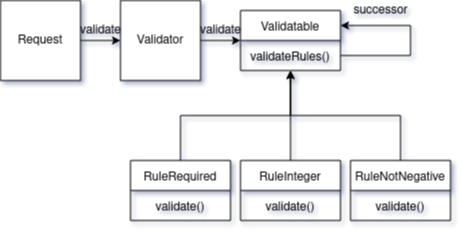
\includegraphics[width=0.75\linewidth]{COR.drawio}
        \caption{graphische Darstellung der Zuständigkeitskette anhand Listing \ref{lst:validator}}
        \label{fig:cor}
    \end{figure}

    Da sich Abb. \ref{fig:cor} direkt auf das Beispiel aus Lst. \ref{lst:validator} bezieht, ist das UML etwas umfangreicher, als die eigentliche Zuständigkeitskette.
    Diese beginnt nämlich erst ab dem Validator selbst.
    Somit werden in \verb|Validatable| die Regeln required, integer und notnegative abgearbeitet.
    Wir nutzen dieses Entwurfsmuster, da eine Validierung von (User-)Input ein sehr repetetiver Vorgang ist.
    Eine Einstiegsklasse als \textit{handler}, welche die einzelnen Regeln abarbeitet erleichtert den Programmieraufand und reduziert die Komplexität des Codes.
    Somit muss bei einer künftigen Erweiterung um weitere Regeln lediglich eine neue Regel-Klasse angelegt werden, welche in \verb|$registeredRulesets| der \verb|Validatable|-Klasse registriert werden müssen.
\end{document}
